\documentclass[11pt,a4paper]{report}
\usepackage[textwidth=37em,vmargin=30mm]{geometry}
\usepackage{calc,xunicode,amsmath,amssymb,paralist,enumitem,tabu,booktabs,datetime2,xeCJK,xeCJKfntef,listings}
\usepackage{tocloft,fancyhdr,tcolorbox,xcolor,graphicx,eso-pic,xltxtra,xelatexemoji}

\newcommand{\envyear}[0]{2025}
\newcommand{\envdatestr}[0]{2025-03-13}
\newcommand{\envfinaldir}[0]{webdb/2025/20250313/final}

\usepackage[hidelinks]{hyperref}
\hypersetup{
    colorlinks=false,
    pdfpagemode=FullScreen,
    pdftitle={Web Digest - \envdatestr}
}

\setlength{\cftbeforechapskip}{10pt}
\renewcommand{\cftchapfont}{\rmfamily\bfseries\large\raggedright}
\setlength{\cftbeforesecskip}{2pt}
\renewcommand{\cftsecfont}{\sffamily\small\raggedright}

\setdefaultleftmargin{2em}{2em}{1em}{1em}{1em}{1em}

\usepackage{xeCJK,xeCJKfntef}
\xeCJKsetup{PunctStyle=plain,RubberPunctSkip=false,CJKglue=\strut\hskip 0pt plus 0.1em minus 0.05em,CJKecglue=\strut\hskip 0.22em plus 0.2em}
\XeTeXlinebreaklocale "zh"
\XeTeXlinebreakskip = 0pt


\setmainfont{Brygada 1918}
\setromanfont{Brygada 1918}
\setsansfont{IBM Plex Sans}
\setmonofont{JetBrains Mono NL}
\setCJKmainfont{Noto Serif CJK SC}
\setCJKromanfont{Noto Serif CJK SC}
\setCJKsansfont{Noto Sans CJK SC}
\setCJKmonofont{Noto Sans CJK SC}

\setlength{\parindent}{0pt}
\setlength{\parskip}{8pt}
\linespread{1.15}

\lstset{
	basicstyle=\ttfamily\footnotesize,
	numbersep=5pt,
	backgroundcolor=\color{black!5},
	showspaces=false,
	showstringspaces=false,
	showtabs=false,
	tabsize=2,
	captionpos=b,
	breaklines=true,
	breakatwhitespace=true,
	breakautoindent=true,
	linewidth=\textwidth
}






\newcommand{\coverpic}[2]{
    % argv: itemurl, authorname
    Cover photo by #2~~(\href{#1}{#1})
}
\newcommand{\makeheader}[0]{
    \begin{titlepage}
        % \newgeometry{hmargin=15mm,tmargin=21mm,bmargin=12mm}
        \begin{center}
            
            \rmfamily\scshape
            \fontspec{BaskervilleF}
            \fontspec{Old Standard}
            \fontsize{59pt}{70pt}\selectfont
            WEB\hfill DIGEST
            
            \vfill
            % \vskip 30pt
            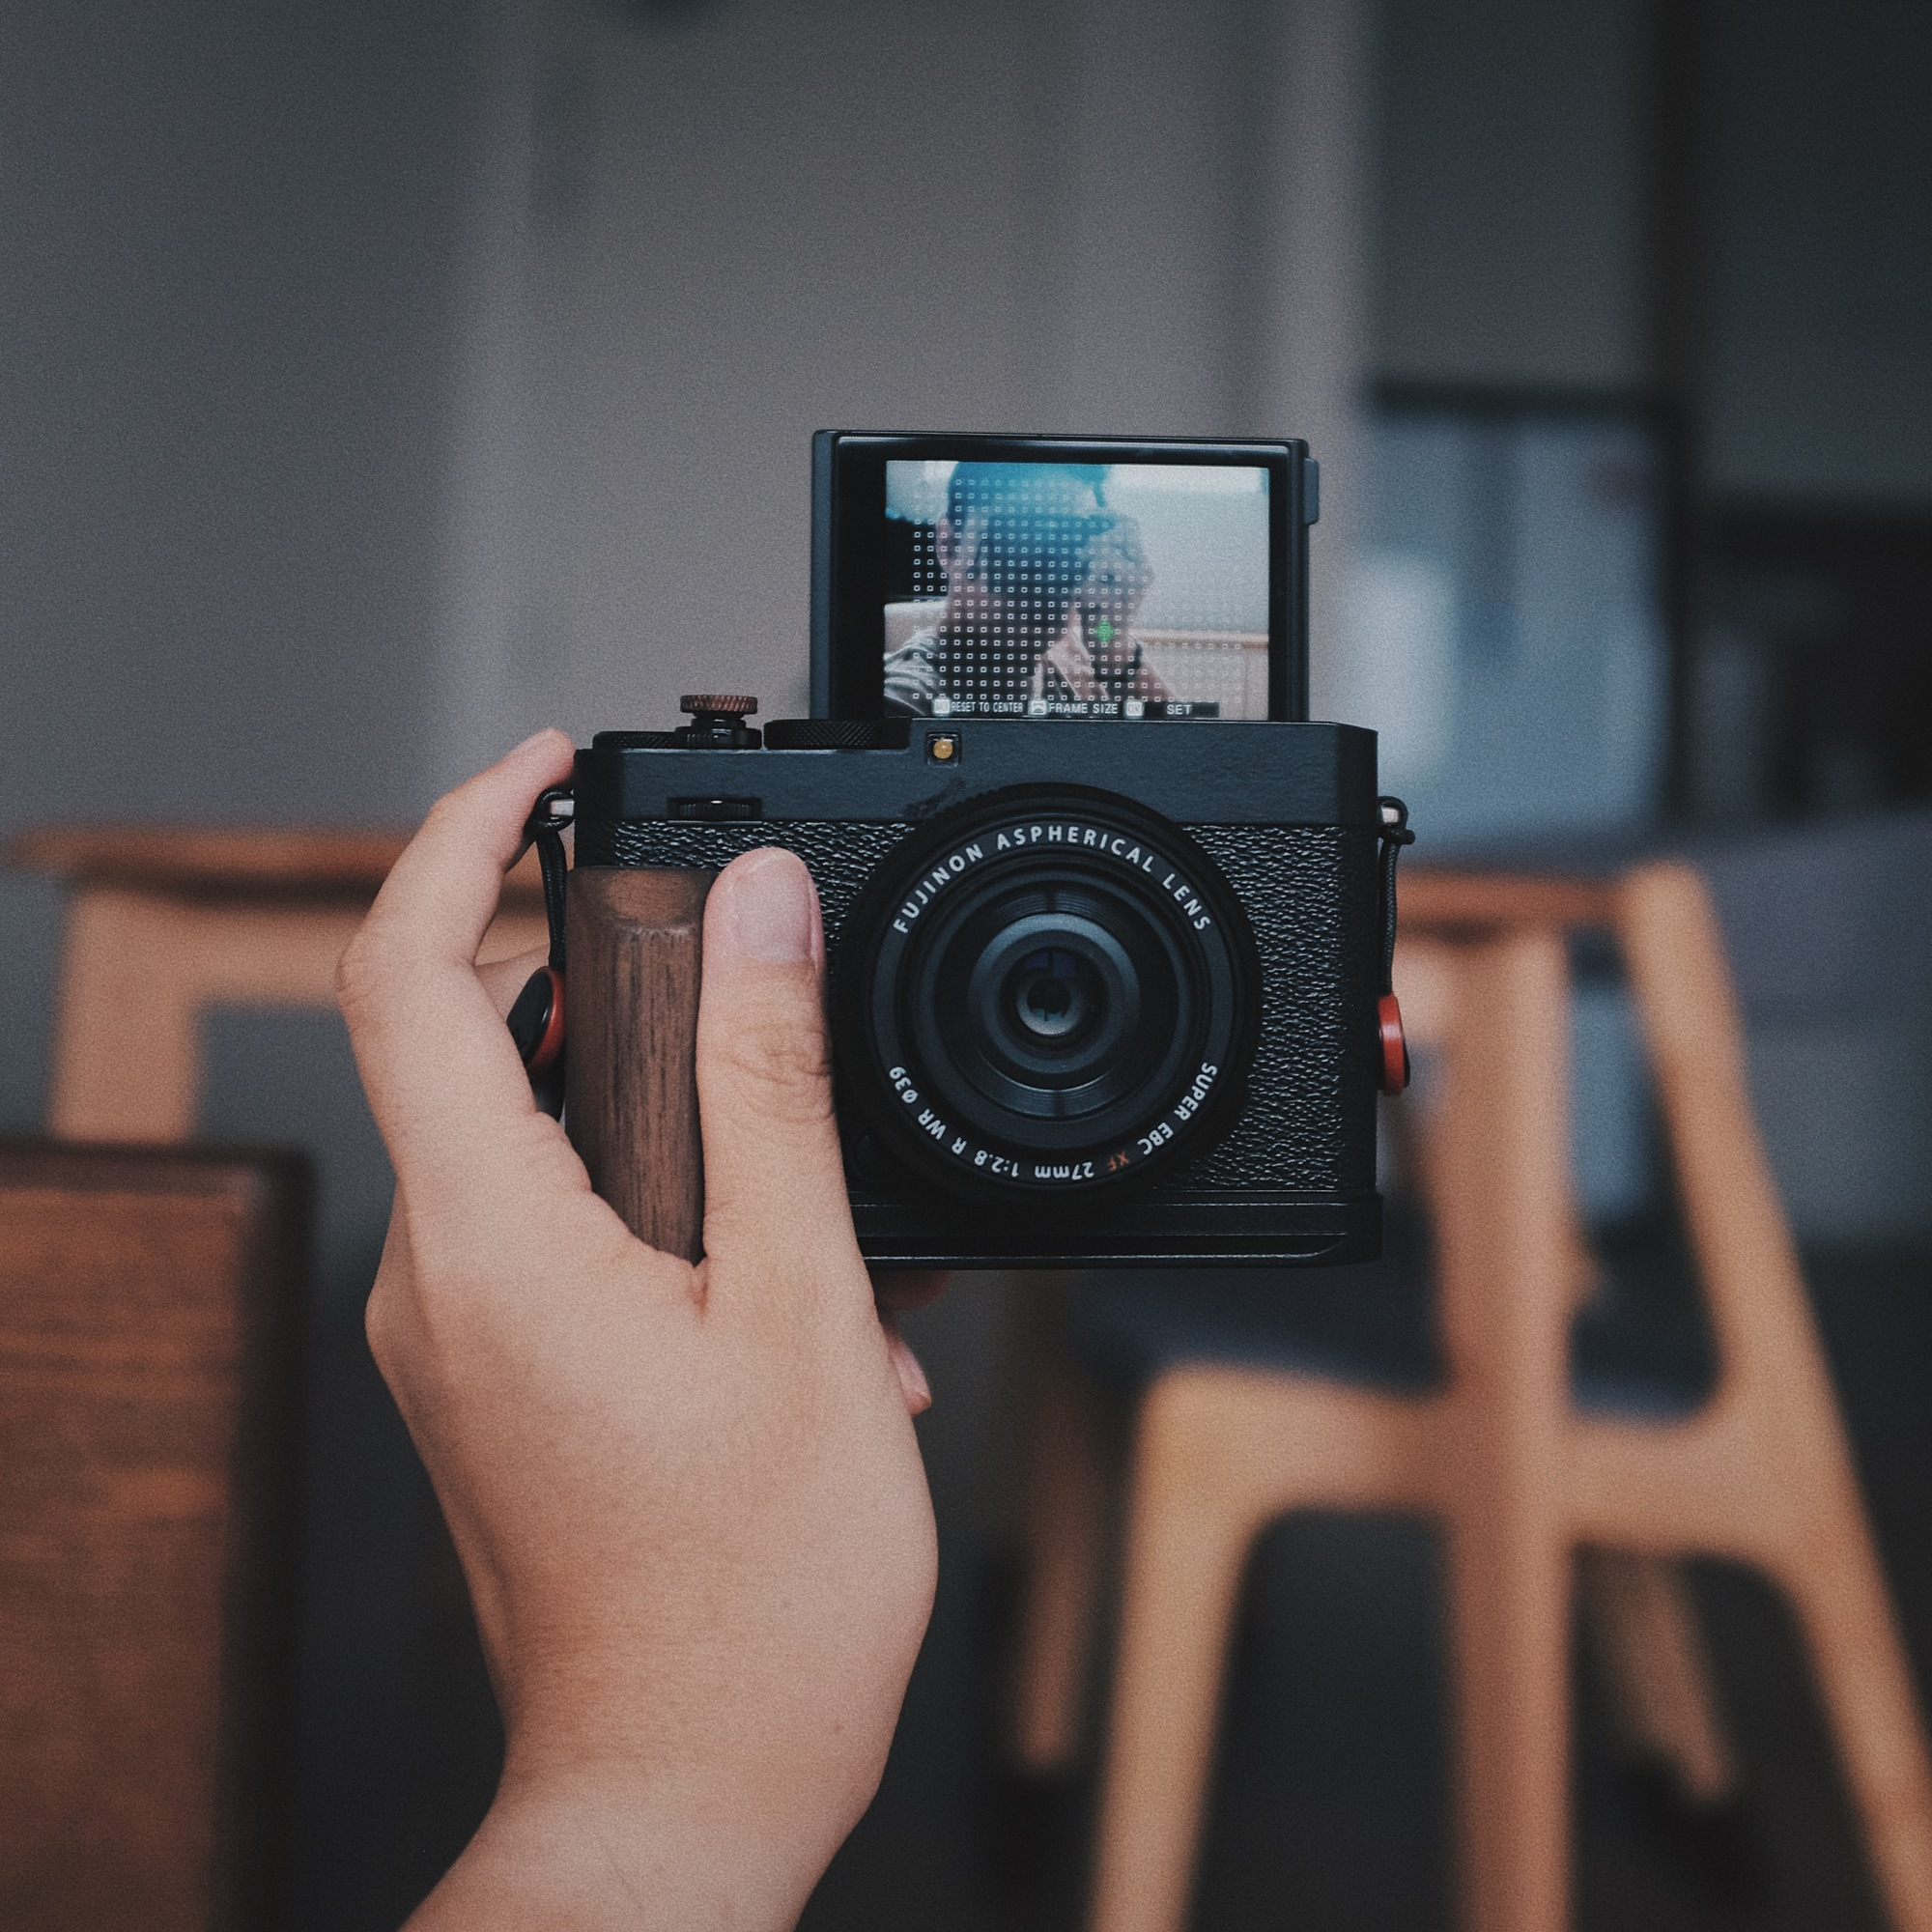
\includegraphics[width=\linewidth]{\envfinaldir/coverpic-prod.jpg}\par
            % \vskip 30pt
            \vfill

            \normalsize\rmfamily\scshape
            \copyright{} The Web Digest Project \hfill\large \envdatestr
        \end{center}
    \end{titlepage}
    % \restoregeometry
}
\newcommand{\simplehref}[1]{%
    \textcolor{blue!80!green}{\href{#1}{#1}}%
}
\renewcommand{\contentsname}{\center\Huge\sffamily\bfseries Contents\par\vskip 20pt}
\newcounter{ipartcounter}
\setcounter{ipartcounter}{0}
\newcommand{\ipart}[1]{
    % \vskip 20pt
    \clearpage
    \stepcounter{ipartcounter}
    \phantomsection
    \addcontentsline{toc}{chapter}{#1}
    % \begin{center}
    %     \Huge
    %     \sffamily\bfseries
    %     #1
    % \end{center}
    % \vskip 20pt plus 7pt
}
\newcounter{ichaptercounter}
\setcounter{ichaptercounter}{0}
\newcommand{\ichapter}[1]{
    % \vskip 20pt
    \clearpage
    \stepcounter{ichaptercounter}
    \phantomsection
    \addcontentsline{toc}{section}{\numberline{\arabic{ichaptercounter}}#1}
    \begin{center}
        \Huge
        \sffamily\bfseries
        #1
    \end{center}
    \vskip 20pt plus 7pt
}
\newcommand{\entrytitlefont}[1]{\subsection*{\raggedright\Large\sffamily\bfseries#1}}
\newcommand{\entryitemGeneric}[2]{
    % argv: title, url
    \parbox{\linewidth}{
        \entrytitlefont{#1}\par\vskip 5pt
        \footnotesize\ttfamily\mdseries
        \simplehref{#2}
    }\vskip 11pt plus 11pt minus 1pt
}
\newcommand{\entryitemGithub}[3]{
    % argv: title, url, desc
    \parbox{\linewidth}{
        \entrytitlefont{#1}\par\vskip 5pt
        \footnotesize\ttfamily\mdseries
        \simplehref{#2}\par\vskip 5pt
        \small\rmfamily\mdseries#3
    }\vskip 11pt plus 11pt minus 1pt
}
\newcommand{\entryitemAp}[3]{
    % argv: title, url, desc
    \parbox{\linewidth}{
        \entrytitlefont{#1}\par\vskip 5pt
        \footnotesize\ttfamily\mdseries
        \simplehref{#2}\par\vskip 5pt
        \small\rmfamily\mdseries#3
    }\vskip 11pt plus 11pt minus 1pt
}
\newcommand{\entryitemHackernews}[3]{
    % argv: title, hnurl, rawurl
    % \parbox{\linewidth}{
    %     \entrytitlefont{#1}\par\vskip 5pt
    %     \footnotesize\ttfamily\mdseries
    %     \simplehref{#3}\par
    %     \textcolor{black!50}{\href{#2}{#2}}
    % }\vskip 11pt plus 11pt minus 1pt
    \begin{minipage}{\linewidth}
            \entrytitlefont{#1}\par\vskip 5pt
            \footnotesize\ttfamily\mdseries
            \simplehref{#3}\par
            \textcolor{black!50}{\href{#2}{#2}}
    \end{minipage}\par\vskip 11pt plus 11pt minus 1pt
}







\begin{document}

\makeheader

\tableofcontents\clearpage




\ipart{Developers}
\ichapter{Hacker News}
\entryitemTwoLinks{Mark Klein, AT\&T whistleblower who revealed NSA mass spying, has died}{https://news.ycombinator.com/item?id=43347662}{https://www.eff.org/deeplinks/2025/03/memoriam-mark-klein-att-whistleblower-about-nsa-mass-spying}

\entryitemTwoLinks{Intel appoints Lip-Bu Tan as its CEO}{https://news.ycombinator.com/item?id=43347369}{https://www.reuters.com/technology/us-chipmaker-intel-appoints-lip-bu-tan-its-ceo-2025-03-12/}

\entryitemTwoLinks{Show HN: Time Portal – Get dropped into history, guess where you landed}{https://news.ycombinator.com/item?id=43347306}{https://www.eggnog.ai/entertimeportal}

\entryitemTwoLinks{Iconography of the PuTTY tools}{https://news.ycombinator.com/item?id=43346816}{https://www.chiark.greenend.org.uk/~sgtatham/quasiblog/putty-icons/}

\entryitemTwoLinks{Shenmue (1999) reverse engineering reveals possible sun position oversight}{https://news.ycombinator.com/item?id=43345285}{https://wulinshu.com/2025/03/11/reverse-engineering-adventures-3-bug-or-not-bug/}

\entryitemTwoLinks{The cultural divide between mathematics and AI}{https://news.ycombinator.com/item?id=43344703}{https://sugaku.net/content/understanding-the-cultural-divide-between-mathematics-and-ai/}

\entryitemTwoLinks{Reverse engineering OpenAI code execution to make it run C and JavaScript}{https://news.ycombinator.com/item?id=43344673}{https://twitter.com/benswerd/status/1899853533761200300}

\entryitemTwoLinks{The 2005 Sony Bravia ad}{https://news.ycombinator.com/item?id=43344129}{https://www.sfgate.com/sf-culture/article/san-francisco-sony-bouncy-ball-ad-20204385.php}

\entryitemTwoLinks{Gemini Robotics}{https://news.ycombinator.com/item?id=43344082}{https://deepmind.google/discover/blog/gemini-robotics-brings-ai-into-the-physical-world/}

\entryitemTwoLinks{The DuckDB Local UI}{https://news.ycombinator.com/item?id=43342712}{https://duckdb.org/2025/03/12/duckdb-ui.html}

\entryitemTwoLinks{Peer-to-peer file transfers in the browser}{https://news.ycombinator.com/item?id=43342361}{https://github.com/kern/filepizza}

\entryitemTwoLinks{The Future Is Niri}{https://news.ycombinator.com/item?id=43342178}{https://ersei.net/en/blog/niri}

\entryitemTwoLinks{First ammonia-fueled ship hits a snag}{https://news.ycombinator.com/item?id=43342071}{https://spectrum.ieee.org/ammonia-fuel-2671266100}

\entryitemTwoLinks{EU to impose counter tariffs on \$28 billion of US goods}{https://news.ycombinator.com/item?id=43341226}{https://www.reuters.com/markets/europe/eu-impose-counter-tariffs-over-28-billion-us-goods-2025-03-12/}

\entryitemTwoLinks{Tell Mozilla: it's time to ditch Google}{https://news.ycombinator.com/item?id=43340948}{https://mozillapetition.com/}

\entryitemTwoLinks{Gemma3 – The current strongest model that fits on a single GPU}{https://news.ycombinator.com/item?id=43340785}{https://ollama.com/library/gemma3}

\entryitemTwoLinks{I stopped everything and started writing C again}{https://news.ycombinator.com/item?id=43340731}{https://www.kmx.io/blog/why-stopped-everything-and-started-writing-C-again}

\entryitemTwoLinks{I use Cursor daily - here's how I avoid the garbage parts}{https://news.ycombinator.com/item?id=43340662}{https://www.nickcraux.com/blog/cursor-tips}

\entryitemTwoLinks{Azure's Weakest Link? How API Connections Spill Secrets}{https://news.ycombinator.com/item?id=43340505}{https://binarysecurity.no/posts/2025/03/api-connections}

\entryitemTwoLinks{Gemma 3 Technical Report [pdf]}{https://news.ycombinator.com/item?id=43340491}{https://storage.googleapis.com/deepmind-media/gemma/Gemma3Report.pdf}\ichapter{Phoronix}
\entryitemGeneric{\hskip 0pt{}Lip-Bu Tan Named As Next Intel CEO}{https://www.phoronix.com/news/Intel-CEO-Lip-Bu-Tan}

\entryitemGeneric{\hskip 0pt{}Ubuntu 25.10 Looks To Make Use Of Rust Coreutils \& Other Rust System Components}{https://www.phoronix.com/news/Ubuntu-25.10-Rust-Coreutils}

\entryitemGeneric{\hskip 0pt{}AMD's 3D V-Cache Optimizer Driver For Squeezing More Ryzen 9 9950X3D Performance}{https://www.phoronix.com/review/amd-3d-vcache-optimizer-9950x3d}

\entryitemGeneric{\hskip 0pt{}OpenSSL 3.5 Alpha 1 Released With Server-Side QUIC}{https://www.phoronix.com/news/OpenSSL-3.5-Alpha-1}

\entryitemGeneric{\hskip 0pt{}AMD Ryzen 9 9900X3D Linux Benchmarks Forthcoming}{https://www.phoronix.com/news/AMD-Ryzen-9-9900X3D-Linux}

\entryitemGeneric{\hskip 0pt{}Linux 6.15 Set To Include Better Handling For Intel P Or E Core Only Mitigations}{https://www.phoronix.com/news/Linux-6.15-P-E-Core-Mitigation}

\entryitemGeneric{\hskip 0pt{}KDE's KWin Wayland \& X11 Code Are Now Split, KWin\_X11 To Be Maintained Until Plasma 7}{https://www.phoronix.com/news/KWin-Wayland-X11-Split}

\entryitemGeneric{\hskip 0pt{}Haiku OS Wrapping Up Its New malloc \& Various Performance Optimizations}{https://www.phoronix.com/news/Haiku-OS-New-malloc-More-Perf}

\entryitemGeneric{\hskip 0pt{}LLVM 20's Great Fortran Language Support With Flang}{https://www.phoronix.com/news/LLVM-20-Flang}\ichapter{Dribbble}
\entryitemGeneric{\hskip 0pt{}Carbon Solutions B2B Dashboard Design}{https://dribbble.com/shots/25681782-Carbon-Solutions-B2B-Dashboard-Design}

\entryitemGeneric{\hskip 0pt{}Fishing Tournament Logo}{https://dribbble.com/shots/25750107-Fishing-Tournament-Logo}

\entryitemGeneric{\hskip 0pt{}Triceratops}{https://dribbble.com/shots/25749787-Triceratops}

\entryitemGeneric{\hskip 0pt{}Atoms - Logo Concepts}{https://dribbble.com/shots/25749091-Atoms-Logo-Concepts}

\entryitemGeneric{\hskip 0pt{}Sergeant Scooper}{https://dribbble.com/shots/25749566-Sergeant-Scooper}

\entryitemGeneric{\hskip 0pt{}Lamar® 21°}{https://dribbble.com/shots/25750164-Lamar-21}

\entryitemGeneric{\hskip 0pt{}Logo For Designed.supply}{https://dribbble.com/shots/25748434-Logo-For-Designed-supply}

\entryitemGeneric{\hskip 0pt{}Codila Studio}{https://dribbble.com/shots/25749456-Codila-Studio}

\entryitemGeneric{\hskip 0pt{}Line Icons}{https://dribbble.com/shots/25749882-Line-Icons}

\entryitemGeneric{\hskip 0pt{}Crystal // Website}{https://dribbble.com/shots/25742820-Crystal-Website}

\entryitemGeneric{\hskip 0pt{}Emergency App Concept Design}{https://dribbble.com/shots/25711688-Emergency-App-Concept-Design}

\entryitemGeneric{\hskip 0pt{}Sway}{https://dribbble.com/shots/25744097-Sway}

\entryitemGeneric{\hskip 0pt{}Partify}{https://dribbble.com/shots/25040893-Partify}

\entryitemGeneric{\hskip 0pt{}ABN-AMRO - Logo Redesign}{https://dribbble.com/shots/25743181-ABN-AMRO-Logo-Redesign}

\entryitemGeneric{\hskip 0pt{}OneC1 - Logo Design}{https://dribbble.com/shots/25732400-OneC1-Logo-Design}

\entryitemGeneric{\hskip 0pt{}Heyo® Monograms}{https://dribbble.com/shots/25732379-Heyo-Monograms}

\entryitemGeneric{\hskip 0pt{}Best Friends}{https://dribbble.com/shots/25730832-Best-Friends}

\entryitemGeneric{\hskip 0pt{}Ecommerce illustration}{https://dribbble.com/shots/25734258-Ecommerce-illustration}

\entryitemGeneric{\hskip 0pt{}Free Fly Apparel}{https://dribbble.com/shots/25727838-Free-Fly-Apparel}

\entryitemGeneric{\hskip 0pt{}Columbus Rapids® C-Wave}{https://dribbble.com/shots/25727535-Columbus-Rapids-C-Wave}

\entryitemGeneric{\hskip 0pt{}Bloodhound Detective}{https://dribbble.com/shots/25726401-Bloodhound-Detective}

\entryitemGeneric{\hskip 0pt{}QLOUD - Logo Redesign}{https://dribbble.com/shots/25726630-QLOUD-Logo-Redesign}

\entryitemGeneric{\hskip 0pt{}Faithful web design}{https://dribbble.com/shots/25723024-Faithful-web-design}

\entryitemGeneric{\hskip 0pt{}Dj Dule logo}{https://dribbble.com/shots/25725864-Dj-Dule-logo}


\ipart{Developers~~~~(zh-Hans)}
\ichapter{Solidot}
\entryitemGeneric{\hskip 0pt{}Spotify 在 2024 年支付了 100 亿美元版税}{https://www.solidot.org/story?sid=80772}

\entryitemGeneric{\hskip 0pt{}Meta 开始测试其自研 AI 训练芯片}{https://www.solidot.org/story?sid=80771}

\entryitemGeneric{\hskip 0pt{}空气污染与生物衰老正相关,而绿地负相关}{https://www.solidot.org/story?sid=80770}

\entryitemGeneric{\hskip 0pt{}台积电提议与 AMD 等接管英特尔芯片制造业务}{https://www.solidot.org/story?sid=80769}

\entryitemGeneric{\hskip 0pt{}全球只有 7 个国家的 PM2.5 水平达到 WHO 的标准}{https://www.solidot.org/story?sid=80768}

\entryitemGeneric{\hskip 0pt{}TP-Link 高危漏洞被僵尸网络感染传播恶意程序}{https://www.solidot.org/story?sid=80767}

\entryitemGeneric{\hskip 0pt{}西班牙将对不标记 AI 生成内容的公司处以巨额罚款}{https://www.solidot.org/story?sid=80766}

\entryitemGeneric{\hskip 0pt{}Firefox 一根证书将于 2025 年 3 月 14 日过期}{https://www.solidot.org/story?sid=80765}

\entryitemGeneric{\hskip 0pt{}新西兰卫生部的财务管理系统是单张 Excel 表格}{https://www.solidot.org/story?sid=80764}

\entryitemGeneric{\hskip 0pt{}科学家发现已知最古老的陨石坑}{https://www.solidot.org/story?sid=80763}

\entryitemGeneric{\hskip 0pt{}研究发现霸凌者有更多孩子}{https://www.solidot.org/story?sid=80762}

\entryitemGeneric{\hskip 0pt{}研究发现微塑料会影响植物的光合作用}{https://www.solidot.org/story?sid=80761}

\entryitemGeneric{\hskip 0pt{}GCC 15 合并了 COBOL 前端}{https://www.solidot.org/story?sid=80760}

\entryitemGeneric{\hskip 0pt{}独生子女政策意外提高了女性的创业率}{https://www.solidot.org/story?sid=80759}

\entryitemGeneric{\hskip 0pt{}温室气体排放或影响人造卫星}{https://www.solidot.org/story?sid=80758}

\entryitemGeneric{\hskip 0pt{}惠普更新打印机固件导致惠普墨盒无法使用}{https://www.solidot.org/story?sid=80757}

\entryitemGeneric{\hskip 0pt{}Eric Sc​​hmidt 成为火箭公司 Relativity Space 的 CEO}{https://www.solidot.org/story?sid=80756}

\entryitemGeneric{\hskip 0pt{}微软计划今年发布 Xbox 掌机,2027 年推出下一代 Xbox 主机}{https://www.solidot.org/story?sid=80755}

\entryitemGeneric{\hskip 0pt{}Google Pixel 4a 存在电池过热风险}{https://www.solidot.org/story?sid=80754}

\entryitemGeneric{\hskip 0pt{}Chrome Store 不再提供 uBlock Origin}{https://www.solidot.org/story?sid=80753}\ichapter{V2EX}
\entryitemGeneric{\hskip 0pt{}[程序员] kafka-server 出问题,删除所有数据,应用客户端没重启, offset 会乱吗}{https://www.v2ex.com/t/1117997}

\entryitemGeneric{\hskip 0pt{}[Notion] 今天收到 Notion Mail 的邮件。}{https://www.v2ex.com/t/1117996}

\entryitemGeneric{\hskip 0pt{}[Linux] 分享个人小项目:把 wireguard client 配置打包成 deb 包}{https://www.v2ex.com/t/1117995}

\entryitemGeneric{\hskip 0pt{}[问与答] 3000 元以内最强半高刀卡显卡推荐?}{https://www.v2ex.com/t/1117994}

\entryitemGeneric{\hskip 0pt{}[Windows] 用一些奇怪的步骤让「不支持的硬件」Win11 收到 24H2 更新}{https://www.v2ex.com/t/1117993}

\entryitemGeneric{\hskip 0pt{}[程序员] 难道只有我中招了 cursor 的 2 刀一次的 GPT4.5 吗}{https://www.v2ex.com/t/1117992}

\entryitemGeneric{\hskip 0pt{}[问与答] 连续几天出去野钓 睡车里}{https://www.v2ex.com/t/1117990}

\entryitemGeneric{\hskip 0pt{}[Java] 新入职遇到极难维护的屎山项目怎么办}{https://www.v2ex.com/t/1117989}

\entryitemGeneric{\hskip 0pt{}[Android] ios 换安卓手机(求推荐}{https://www.v2ex.com/t/1117986}

\entryitemGeneric{\hskip 0pt{}[问与答] 这是一个求助关于如何在 dos 模式下升级主板的 Phoenix Award BIOS 来解决已知问题}{https://www.v2ex.com/t/1117985}

\entryitemGeneric{\hskip 0pt{}[Android] Android 系统重建 Activity 时为什么不重建 Intent?}{https://www.v2ex.com/t/1117984}

\entryitemGeneric{\hskip 0pt{}[这个世界不完美] QQ 邮箱的``文件云盘''服务条款长达四个字}{https://www.v2ex.com/t/1117979}

\entryitemGeneric{\hskip 0pt{}[程序员] 论腾讯小程序备案初审工作人员的文化水平是否达到了初中毕业水平?}{https://www.v2ex.com/t/1117978}

\entryitemGeneric{\hskip 0pt{}[分享创造] [开源导航] 小红书独立开发者大赛导航页,写一半不想写了,开源了}{https://www.v2ex.com/t/1117977}

\entryitemGeneric{\hskip 0pt{}[分享创造] 小组件上新啦,欢迎体验}{https://www.v2ex.com/t/1117974}

\entryitemGeneric{\hskip 0pt{}[程序员] 各位 Android 开发大佬,帮忙看看我这个 pixel ims 修改哪里有问题,想用 shizuku 打开 vowifi}{https://www.v2ex.com/t/1117972}

\entryitemGeneric{\hskip 0pt{}[生活] 中年男人的快乐}{https://www.v2ex.com/t/1117970}

\entryitemGeneric{\hskip 0pt{}[问与答] 是我老了,还是新同事很牛?}{https://www.v2ex.com/t/1117969}

\entryitemGeneric{\hskip 0pt{}[Python] Nodezator}{https://www.v2ex.com/t/1117967}

\entryitemGeneric{\hskip 0pt{}[程序员] 35+大龄程序员,刚生娃,即将被裁,该怎么办}{https://www.v2ex.com/t/1117966}

\entryitemGeneric{\hskip 0pt{}[酷工作] 广州 | Android 开发招聘}{https://www.v2ex.com/t/1117965}

\entryitemGeneric{\hskip 0pt{}[程序员] 跨端 APP 数据同步问题}{https://www.v2ex.com/t/1117963}

\entryitemGeneric{\hskip 0pt{}[问与答] 求助 : 校内网络无法 ssh 连接学校服务器}{https://www.v2ex.com/t/1117962}

\entryitemGeneric{\hskip 0pt{}[职场话题] 身为面试官如何能 找出来匹配的候选人}{https://www.v2ex.com/t/1117960}

\entryitemGeneric{\hskip 0pt{}[AirPods] AirPods 4 降噪版值得入手吗}{https://www.v2ex.com/t/1117959}

\entryitemGeneric{\hskip 0pt{}[问与答] 想学画画(日系),但是没有方向,有没有大佬给点指导?}{https://www.v2ex.com/t/1117958}

\entryitemGeneric{\hskip 0pt{}[程序员] 求助 X99 平台跑 PVE8 的 Windows 虚拟机整个电脑宕掉的问题}{https://www.v2ex.com/t/1117957}

\entryitemGeneric{\hskip 0pt{}[宽带症候群] 放弃折腾,大道至简}{https://www.v2ex.com/t/1117956}

\entryitemGeneric{\hskip 0pt{}[Surge] 有没有出 surge for mac 授权的,收一个,麻烦留下小而美}{https://www.v2ex.com/t/1117955}

\entryitemGeneric{\hskip 0pt{}[问与答] 汽水音乐这是在干嘛?}{https://www.v2ex.com/t/1117954}

\entryitemGeneric{\hskip 0pt{}[分享创造] 做了个用户无侵入的浏览器书签管理插件}{https://www.v2ex.com/t/1117953}

\entryitemGeneric{\hskip 0pt{}[Ubuntu] 求 Ubuntu 台式机指纹 USB 识别器推荐}{https://www.v2ex.com/t/1117952}

\entryitemGeneric{\hskip 0pt{}[Next.js] drizzle 中 many-to-many 的表怎么插入更优雅}{https://www.v2ex.com/t/1117951}

\entryitemGeneric{\hskip 0pt{}[NAS] 记一次安装 fnOS 失败}{https://www.v2ex.com/t/1117950}

\entryitemGeneric{\hskip 0pt{}[分享创造] 代码小白花了 3 个小时,开发了一个物联网用的 MCP Server,现已 Apache2.0 开源}{https://www.v2ex.com/t/1117949}

\entryitemGeneric{\hskip 0pt{}[分享创造] 用 AI 给 b 站写了个油猴脚本(随机播放列表,自定义倍速等)}{https://www.v2ex.com/t/1117948}

\entryitemGeneric{\hskip 0pt{}[C++] 有人遇到过 vs2022 c++代码高亮不生效的问题吗?}{https://www.v2ex.com/t/1117947}

\entryitemGeneric{\hskip 0pt{}[分享创造] 给你的 JSON 穿上"锦衣":让杂乱无章的数据焕然一新!}{https://www.v2ex.com/t/1117946}

\entryitemGeneric{\hskip 0pt{}[酷工作] 华侨银行内推}{https://www.v2ex.com/t/1117944}

\entryitemGeneric{\hskip 0pt{}[程序员] 有没有便利的认证和解锁集成方案(windows hello)?}{https://www.v2ex.com/t/1117943}

\entryitemGeneric{\hskip 0pt{}[宽带症候群] 因群晖开了 qc 再次被电信警告了}{https://www.v2ex.com/t/1117942}

\entryitemGeneric{\hskip 0pt{}[程序员] [MoonBit OJ 编程竞赛-选拔赛] 参与了初赛,成功拿了 500 块}{https://www.v2ex.com/t/1117940}

\entryitemGeneric{\hskip 0pt{}[宽带症候群] 北京联通把 pppoe 双拨给禁了?}{https://www.v2ex.com/t/1117939}

\entryitemGeneric{\hskip 0pt{}[求职] 24 届前端想找一份 remote 工作}{https://www.v2ex.com/t/1117938}

\entryitemGeneric{\hskip 0pt{}[程序员] 求推荐 JetBrains Mono 的变体字体}{https://www.v2ex.com/t/1117936}

\entryitemGeneric{\hskip 0pt{}[问与答] Youtube 上评论区经常出现的这种加密货币助记词的评论是什么意思}{https://www.v2ex.com/t/1117934}

\entryitemGeneric{\hskip 0pt{}[职场话题] 编程工作中碰到难缠问题你们是会死磕还是避开}{https://www.v2ex.com/t/1117933}

\entryitemGeneric{\hskip 0pt{}[问与答] 求助,美区 paypal 怎么提现}{https://www.v2ex.com/t/1117931}

\entryitemGeneric{\hskip 0pt{}[生活方式] 脱发可以植发,白发真没救了么?}{https://www.v2ex.com/t/1117930}

\entryitemGeneric{\hskip 0pt{}[问与答] 独立开发者可否开发 AI 工具软件?搞一个中文 Cursor, Chinese LangChain 怎么样?}{https://www.v2ex.com/t/1117929}


\ipart{Generic News}







\clearpage
\leavevmode\vfill
\footnotesize

Copyright \copyright{} 2023-2025 Neruthes and other contributors.

This document is published with CC BY-NC-ND 4.0 license.

The entries listed in this newsletter may be copyrighted by their respective creators.

This newsletter is generated by the Web Digest project.

The newsletters are also delivered via Telegram channel \CJKunderline{\href{https://t.me/webdigestchannel}{https://t.me/webdigestchannel}}.\\
RSS feed is available at \CJKunderline{\href{https://webdigest.pages.dev/rss.xml}{https://webdigest.pages.dev/rss.xml}}.

This newsletter is available in PDF at
\CJKunderline{\href{https://webdigest.pages.dev/}{https://webdigest.pages.dev/}}.

The source code being used to generate this newsletter is available at\\
\CJKunderline{\href{https://github.com/neruthes/webdigest}{https://github.com/neruthes/webdigest}}.

This newsletter is also available in
\CJKunderline{\href{http://webdigest.pages.dev/readhtml/\envyear/WebDigest-20250313.html}{HTML}} and
\CJKunderline{\href{https://github.com/neruthes/webdigest/blob/master/markdown/\envyear/WebDigest-20250313.md}{Markdown}}.


\coverpic{https://unsplash.com/photos/an-aerial-view-of-a-beach-and-ocean-IVAWeeLReb8}{Alim}


\end{document}
